\section{Umsetzungskonzept für die digitale Transformation}

Für die Beantwortung der Forschungsfragen (s. Kapitel \ref{problemstellung}) wurde im Kapitel \ref{losung} ein Lösungsansatz bereits vorgestellt. In dem folgendem Kapitel wird die Umsetzung des Lösungansatzes dargestellt. Zuerst wird ein repräsentativer Anwendungsfall für die Energiewirtschaft entwickelt. Für die Spezifikation der Zielarchitektur des Prototypen wird vorher eine detaillierte Anforderungsanalyse durchgeführt. Außerdem wird vorher eine Systemanalyse der zugrundleliegenden Systemarchitektur von SAP Leonardo durchgeführt. Auf Basis dieser Schritte wird schließlich die das System des Prototypen entworfen und umgesetzt. 

 \subsection{Repräsentativer Anwendungsfall für die Energiewirtschaft}\label{usecase}

Die verschiedenen Werttreiber und Anforderungen für ein Digitalisierungskonzept unterscheiden sich je nach Unternehmen und Branche.
Für eine erfolgreiche Transformation müssen daher individuelle Anwendungsfälle identifziert werden.
In Anbetracht der Dynamik und des rasanten Tempos, in der neue Technologien entstehen,
ermöglicht ein anwendungsfallbasierter Ansatz eine flexible und agile Anpassung. \citep[S. 31]{Acharya2019}
\\Aus diesen Gründen wird im Folgenden ein repräsentativer Anwendungsfall für die Energiebranche vorgestellt. Die Anforderungen an das Zielsystem werden nach den von \citet{Lauenroth2016} vorgestellten Methoden erhoben.

\subsubsection{Ausgangssituation} \label{usecase}

Der deutsche Windenergieanlagenhersteller Enercon GmbH aus Aurich ist mit über 29000 Anlagen in 45 Ländern ein Global Player in der Branche. Da das Kerngeschäft des Unternehmens auf dezentraler Energieproduktion basiert, hat Industrie-4.0-Fähigkeit einen besonderen Stellenwert. Sei es die Einspeisung der produzierten Energie in das Smart-Grid, die Fernsteuerung oder die Zustandsüberwachung der Anlagen und Windparks: Das unternehmenseigene \acf{scada}-System ist auf die Enercon-Anlagen abgestimmt bietet umfangreiche Lösungen für die Kunden. Als Kunden stehen die Energieversorgungsunternehmen im Vordergrund, welche sowohl auf Anforderungen der Netzbetreiber als auch der eigenen Kunden, also der Konsumenten, reagieren müssen. Im Kontext des Unbundlings des Energiemarktes etablierte sich die Branchenlösung \acf{sapisu}, welches Bestandteil von SAP ERP ist, als Vertriebs- und Informationssystem für \ac{evu}. Auch die Enercon-IT nutzt SAP-Produkte für das Management der Ressourcen, Logistik oder Kunden. Im Zuge der Anpassung an die Anforderungen der digitalen Welt wird SAP jedoch den Support der bisher auch von Enercon verwendeten Standard-ERP-Software bis 2025 einstellen. Der Fokus wird auf das Nachfolgeprodukt SAP S/4 HANA gesetzt, welche die echtzeitfähige In-Memory-Datenbanktechnologie \acf{hana} für nutzt. Aus dem Grund bereitet sich Enercon rechtzeitig auf die Migration auf S/4 HANA vor. Die Integrations- und Entwicklungsplattform von \ac{hana} bietet zahlreiche Möglichkeiten zur Realisierung von innovativen Softwarelösungen sowohl auf der Cloud als auch On-Premise. Die Neuausrichtung der IT-Architektur ist auch für die erfolgreiche digitale Transformation von Enercon großer Bedeutung.

\noindent Im besonderen Interesse liegt die SAP Leonardo \ac{iot} Foundation, vor allem in Anbetracht einer möglichen Integration von Stammdaten aus dem S/4 HANA System. Dafür ist zunächst eine Analyse der SAP Leonardo Systemarchitektur mitsamt der Perspektiven gewünscht. Dies könne als Entscheidungsgrundlage für eine Erweiterung des Geschäftsfeldes von Energieproduktion auf IT-Dienstleistungen dienen. Außerdem soll prototypisch dargestellt werden, inwiefern sich SAP Leonardo IoT als Verwaltungsschale für die Industrie-4.0-Komponente eignet. Langfristiges Ziel des Unternehmens sei es, das \ac{scada}-System über die Kommunikationsschnittstelle mit dem OPC XML-DA Protokoll echtzeitfähig zu gestalten. Um Risiken vor Inbetriebnahme und Kosten zu minimieren soll jedoch zunächst eine einfache Simulation genügen.

\noindent Die Simulation soll dem Servicepersonal in der Wartung ermöglichen, die Zustandsdaten des digitalen Zwillings einer Anlage in Echtzeit zu überwachen. Wenn kritische Messwerte empfangen werden, soll das Personal sofort benachrichtigt werden, damit Wartungsmaßnahmen eingeleitet werden können. Die Softwareentwickler/innen sollen den Prototypen beliebig sowohl um (Mess-)Geräte als auch um App-Funktionalitäten erweitern können.

\subsubsection{Anforderungserhebung}

Um die Anforderungen für die Umsetzung einer repräsentativen Lösung zu bestimmen, muss zunächst ermittelt werden, welche Einflussfaktoren sich im Kontext des Zielsystems befinden und wo sich die Grenze des Systems befindet. Mit der Evaluation der Ausgangssituation (s. \ref{usecase}) können Anforderungsquellen identifiziert werden, welche sich auf das Zielsystem beziehen und sich im Systemkontext befinden (s. Abbildung \ref{kontext}). Auf Grundlage der Evaluation werden zunächst Probleme, Anforderungen und Lösungen für das Gesamtsystem definiert. Für eine bessere Strukturierung des Systems werden die einzelnen \ac{pal} auf die Ebenen System und Systemkontext, sowie auch auf die technologische Ebene abstrahiert. Die Dokumentation von Anforderungen auf verschiedenen Abstraktionsebenen ist vor allem für die nachträgliche Verwaltung der Anforderungen für zukünftige Softwareprojekte von großem Wert \citep{Lauenroth2016}. Nach \citet{IREB2017} unterscheidet man typischerweise zwischen drei Arten von Anforderungen: funktionale Anforderungen, Qualitätsanforderungen sowie Randbedingungen. Die funktionalen Anforderungen werden weiter in verschiedene Perspektiven unterteilt. Aus der Struktur- bzw. Datenverspektive wird die Struktur der Ein- und Ausgabedaten beschrieben, welche in der Funktionsperpektive verarbeitet werden. Die Verhaltensperspektive beschreibt das Verhalten des Systems auf Basis von Zuständen und Ereignissen \citep{Lauenroth2016}.
Daraufhin werden aus den ermittelten Anforderungen Teilsysteme identifiziert, für welche die Anfoderungen ebenfalls nach dem \ac{pal}-Model erfasst werden. Die Formulierung von Anforderungen setzt das Vorhandensein einer Lösung voraus, weshalb auch der Prototyp bereits als Anforderungsquelle gelten kann.
\\\\Aus der Evaluation der Ausgangssituation ergibt sich die in Abbildung \ref{kontext} dargestellte Systemabgrenzung. Die Anforderungsanalyse berücktsichtigt die Stakeholder, welche sowohl mit dem System interagieren als auch direkten Einfluss auf die Anforderungen haben. Als Nutzer des Systems kristallisieren sich die Kunden Enercons (z.B. die \ac{evu}) sowie das Servicepersonal, welches in der Wartung tätig ist. Für das Servicepersonal wurden Anwendungsfälle konkretisiert, welche wichtige Anforderungsquellen sind. Stakeholder, welche eher qualitative Anforderungen an das System stellen, sind die Softwareentwickler/innen und -architekt(inn)en, für welche der Prototyp als Architekturvorlage dienen soll. Die Auftraggeber stellen die direkte Anforderung, eine Lösung und Analyse für SAP Leonardo zu entwickeln, die die Eignung SAP Leonardos als Verwaltungsschale für die Industrie-4.0-Komponente beurteilt. Dies impliziert, dass sich an der IT-Sicht (s. Abbildung \ref{it_layer}) der Referenzarchitektur RAMI 4.0 orientiert werden soll. Bereits existierende Systeme können ebenfalls Einfluss auf das System haben, was jedoch für die Prototypentwicklung nicht relevant ist.


\begin{figure}[h]
  \centering
  \includegraphics[width=1\linewidth]{System_Kontext.png}
  \caption[Systemabgrenzung und Systemkontext]{Systemabgrenzung und Systemkontext}
  \label{kontext}
\end{figure}

% Anforderungsanalyse ***********

\subsection{Anforderungsanalyse}

Zielsetzung der vorliegenden Anforderungsanalyse, Aufbau der Analyse, Einführung in das Fachgebiet und offene Punkte -> Die Anforderungsanalyse wird nach dem PAL-MOdell auf die verschiedenen Abstraktionsebenen eines Systems durchgeführt.

\begin{table}[h]
  \begin{tabular}{ p{5cm}|p{5cm}|p{5cm} }
    \toprule
    Problem & Anforderung & Lösung \\
    \midrule
    \multicolumn{3}{ l }{\textbf{Kontextebene} }\\
    \hline
    K-P-1: Problem & K-QA-1: Qualitative Anforderung \newline K-FA-1: Funktionale Anforderung \newline K-RA-1: Randbedingung  & K-L-1: Lösung\\
    \hline
     \multicolumn{3}{ l }{\textbf{Systemebene} }\\
     \hline
     S-P-1: Problem & S-A-1  & S-L-1: Lösung\\
  \hline
    \multicolumn{3}{ l }{\textbf{Technische Ebene} }\\
    \hline
    T-P-1: Problem & T-A-1: Anfoderung  & T-L-1: Lösung\\
    \bottomrule
    \end{tabular}
    \label{pal_table}
  \caption{PAL-Tabelle}
\end{table}

\subsubsection {Kontextebene}



Use Cases ermitteln und aufschreiben
RAMI 4.0 Verwaltungsschale Anforderungen finden

\begin{figure}[h]
  \centering
  \includegraphics[width=1\linewidth]{use_case_diagram.png}
  \caption[Use Case Diagram]{Use Case Diagram -> noch nicht fertig}
  \label{kontext}
\end{figure}

\subsubsection{Systemebene}

Anpassbar, Änderbar, Benutzbar, Genau, Performanz, Sicherheit, Übertragbarkeit, Zuverlässigkeit

Datenflussdiagramm
\subsubsection{Technologische Ebene}





Was muss das System können? An RAMI orientieren -> Was muss erfüllt werden ?
Scada macht über Protokolle und Schnittstellen Telemetriedaten der Windenergieanlage
schreibt das Lokal in eine DB und erzeugt Alarmmeldungen
quittieren lokal am Rechner
alle 10 Minuten --> mit Leonardo schnellere Reaktion in Echtzeit
50 Hz Frequenz -> muss gehalten werden, um schnell auf Probleme reagieren zu können


\begin{itemize}
  \item erneuerbare Energien werden von der Plattform Industrie 4.0 kaum berücksichtigt !
  \item Was Kann SCADA-System? daten erfassen, an cloud senden, verarbeiten, digitaler zwilling unf steuern, aktionen und regeln für predictive Maintenance
  \item Fähigkeit, große Datenmengen auch offline zu verarbeiten -> Latenzprobleme
  \item ANFORDERUNG! WENN DIE Anlagen ins Smart Grid aufgenommen werden sollen, müssen sie Kommunikationsfähig sein!!!!
  \item Aus Requirements Engineering S. 10: Simulation vor Inbetriebnahme, um Fehler in Anforderungsanalyse festzustellen, damit Change Requests gemacht werden können
  \item Bei Anlagen, die mehrere Millionen Euro kosten, sind anders als in Software Mechanik und Elektronik eingebaut. Ein Change Request wäre viel zu teuer
  \item Anforderungsanalyse der Simulation beseitigt die Risiken nicht vollständig, da die Simulation nur so gut ist, wie man sich vorher Gedanken gemacht hat
  \item Welche Anforderungen ergeben sich aus dem Wandel?
  \item Anforderungen wie predictive Maintenance und Bezug auf RAMI 4.0.
  \item SAP als Tool, da Energiesektor hauptsächlich \acf{sapisu}
  \item Industrie 4.0-Komponente (Bitkom s. 52) mit verschiedenen Ebenene
\end{itemize}

\textbf{Anforderungen an Versorgungsunternehmen im Energiesystem der Zukunft \citep[S. 19]{Doleski2016}}

\paragraph{Merkmale von Akteuren in der digitalen Welt}
\begin{itemize}
  \item Allgegenwärtige Informationsverfügbarkeit
  \item Soziale Visualisierung1
  \item Absolute Mobilität
  \item Permanente Erreichbarkeit
  \item Lokalisierung
  \item Leistungsfähige Technologien
\end{itemize}

\paragraph{Wesentliche Herausforderungen für Energieunternehmen \citep[S. 21]{Doleski2016}}
\begin{enumerate}
  \item \textbf{Informationsflut}: zunehmendes Informationsangebot kann nicht oder nur bedingt aufgenommen werden
  \item \textbf{Informationsverarbeitung}: zunehmendes Informationsangebot kann nicht zu Wissen verarbeitet werden
  \item \textbf{Informationssysteme}: bestehende Informationssysteme liefern oftmals keine relevanten Informationen für die Unternehmensführung
\end{enumerate}
%


\paragraph{Einige Anforderungen an Versorgungsunternehmen}
Die Anforderungen sollen sich nur auf die Befähiger/Enabler sowie die Prozesse der Energieunternehmen beziehen
\begin{enumerate}
  \item Im Wettbewerb um geeignete Fachkräfte und Digital Natives bestehen $[Enabler]$
  \item Aufbau eines leistungsfähigen Informationsmanagements zur Speicherung, Verarbeitung und Auswertung sehr großer Datenmengen in Echtzeit $[Enabler]$
  \item Big Data beherrschen und innovative technische Lösungen anbieten $[Enabler]$
  \item Image eines verantwortungsbewusst handelnden Unternehmens schaffen und glaubhaft leben $[Enabler]$
  \item Kosteneffizient und professionell handeln $[Prozesse]$
  \item Veränderung von Organisation und Betriebsprozessen zügig vorantreiben $[Prozesse]$
  \item Alle Abläufe müssen modernen Datensicherheitsanforderungen entsprechen $[Prozesse]$
  \item uvm
\end{enumerate}

 \subsection{Systementwurf und -analyse}
Systementwurf: Hier mein angepasstes Architekturmodell -> konkretes Architekturmodell mit Sensoren, Edge Device (RPI), SCP (CF) mit Leo IoT Services; AWS SNS mit API-Schnittstellen
\\Hier irgendwo auch anmerken in Bezug auf 2.3.3 SAP Leonardo und in der Evaluation ausführlicher vllt, dass zwar der Mehrwert in kombinierter Anwendung besteht, man hier aufgrund einer prototypischen Implementierung und es Bezugs auf IoT nur auf ein Leo-Produkt bezogen wird

\subsubsection{Systemarchitektur}

hier generelle Architektur von SAP Leonardo mit SCP

SOA - Service Orientierte Architektur
\begin{figure}[H]
    \centering
    \includegraphics[width=1.0\linewidth]{pictures/sap_architecture}
    \caption[Referenzarchitektur von SAP]{Architektur von SAP \citep{Ganz2019}}
    \label{fig:filename_without_extension}
\end{figure}


\subsubsection{REST API}

\subsubsection{Edge-Processing}

Protokolle der Edge Server CoAP, File, Modbus, MQTT, OPC UA, REST, SigFox, SNMP
\subsubsection{Destinations}
Destinations: Warum braucht man Destinations und welche man benötigt (SNS),  wenn man kommunizieren will mit
Externe Services wie AWS SNS
Interne Kommunikation der SCP CF und NEO
Communication zwischen Cloud Services AWS SNS und SAP Leonardo

\subsubsection{Message Processing}
Leonardo IoT, SQL Kafka: Ich hab Leonardo IoT benutzt (in prototype erwähnen)

\subsubsection{Sicherheit}
OAuth, SSL/TLS, SAML 2.0: erklären, was SAP und AWS auch eventuell haben

\subsubsection{Systementwurf gemäß Architekturkonzept}

 

\subsection{Prototypische Implementierung des Anwendungsfalls}

In diesem Kapitel wird die Umsetzung des entwickelten Prototypen im Detail beschrieben.
Zunächst wird die Erzeugung eines cyberphysischen Systems als Industrie-4.0-Komponente beschrieben. Im Anschluss wird dargestellt, wie Daten des Messinstruments über die \textit{Internet of Things Edge Platform} an die SAP Cloud Platform übergeben werden. Daraufhin wird die Erzeugung eines digitalen Zwilllings und die Zuordnung von Funktionen beschrieben. Abschließend wird dargestellt, wie der Zustand der Anlage den Nutzern in einer UI5-Applikation präsentiert werden.

\subsubsection{Erzeugung eines cyberphysischen Systems}

Für die Simulation einer Windergieanlage wird ein System erzeugt, welches Daten aus der Umwelt aufnehmen und verarbeiten kann. Bei den Daten wurde sich für die \textit{Windgeschwindigkeit, Temperatur, Luftfeuchtigkeit, Luftdruck und Luftdichte} entschieden.
Als hardwareseitige Basis für die Simulation wird ein \textit{Raspberry Pi 3 B} verwendet, welcher die erstellten \textit{Python} Skripte zur Verarbeitung der Daten nutzt. Der Pi wurde um die Zusatzplatine \textit{Grove Pi + Board} erweitert. Somit wird der \textit{DHT11}-Sensor zur Messung von Temperatur und Luftfeuchtigkeit über die 4-Pin-Schnittstelle \textit{D4} einfach ohne Löten und Breadboard angebunden. Für die Messung der Windgeschwindigkeit ist die Entscheidung auf den Anemometer \textit{Eltako Windsensor WS} gefallen. Im Gegensatz zum \textit{DHT11-Sensor} ist der Anenometer ein aktives Mechanisches Gerät, dessen Output Berechnungen erfordert, um die Windgeschwindigkeit zu erhalten. Bei den ausgegebenen Signalen handelt es sich um die Berührung zweier Metallkontakte, wobei zwei Signale eine Umdrehung ergeben. Ein Python Skript zählt die Signale über der GPIO-4-Schnittstelle und berechnet die Geschwindigkeit für ein Zeitintervall von 5 Sekunden. Aufgrund mangelhafter Sensorik wird der Luftdruck aus einem Array von realistischen Werten zufällig pro Zeitintervall ausgewählt. Gemeinsam mit der gemessenen Temperatur und dem Luftdruck wird die Luftdichte berechnet. Bevor die Daten an das Gateway gesendet werden, werden sie dem String-Dictionary \textit{sensorData} übergeben, um eine Anfrage im \textit{JSON-Format} senden zu können. Außerdem wurde eine rote Grove-LED über die digitale Schnittstelle D3 angebunden. Diese Komponente dient im Gegensatz zu den weiteren Komponenten dazu, bei kritischen Temperaturwerten Befehle zum Aufleuchten zu erhalten. Damit soll gezeigt werden, dass sich der Kreis in einem cyberphysischen System von Sensorik bis Aktorik über SAP Leoanardo als informationsverarbeitende Schicht schließt.

\begin{figure}[H]
  \centering
  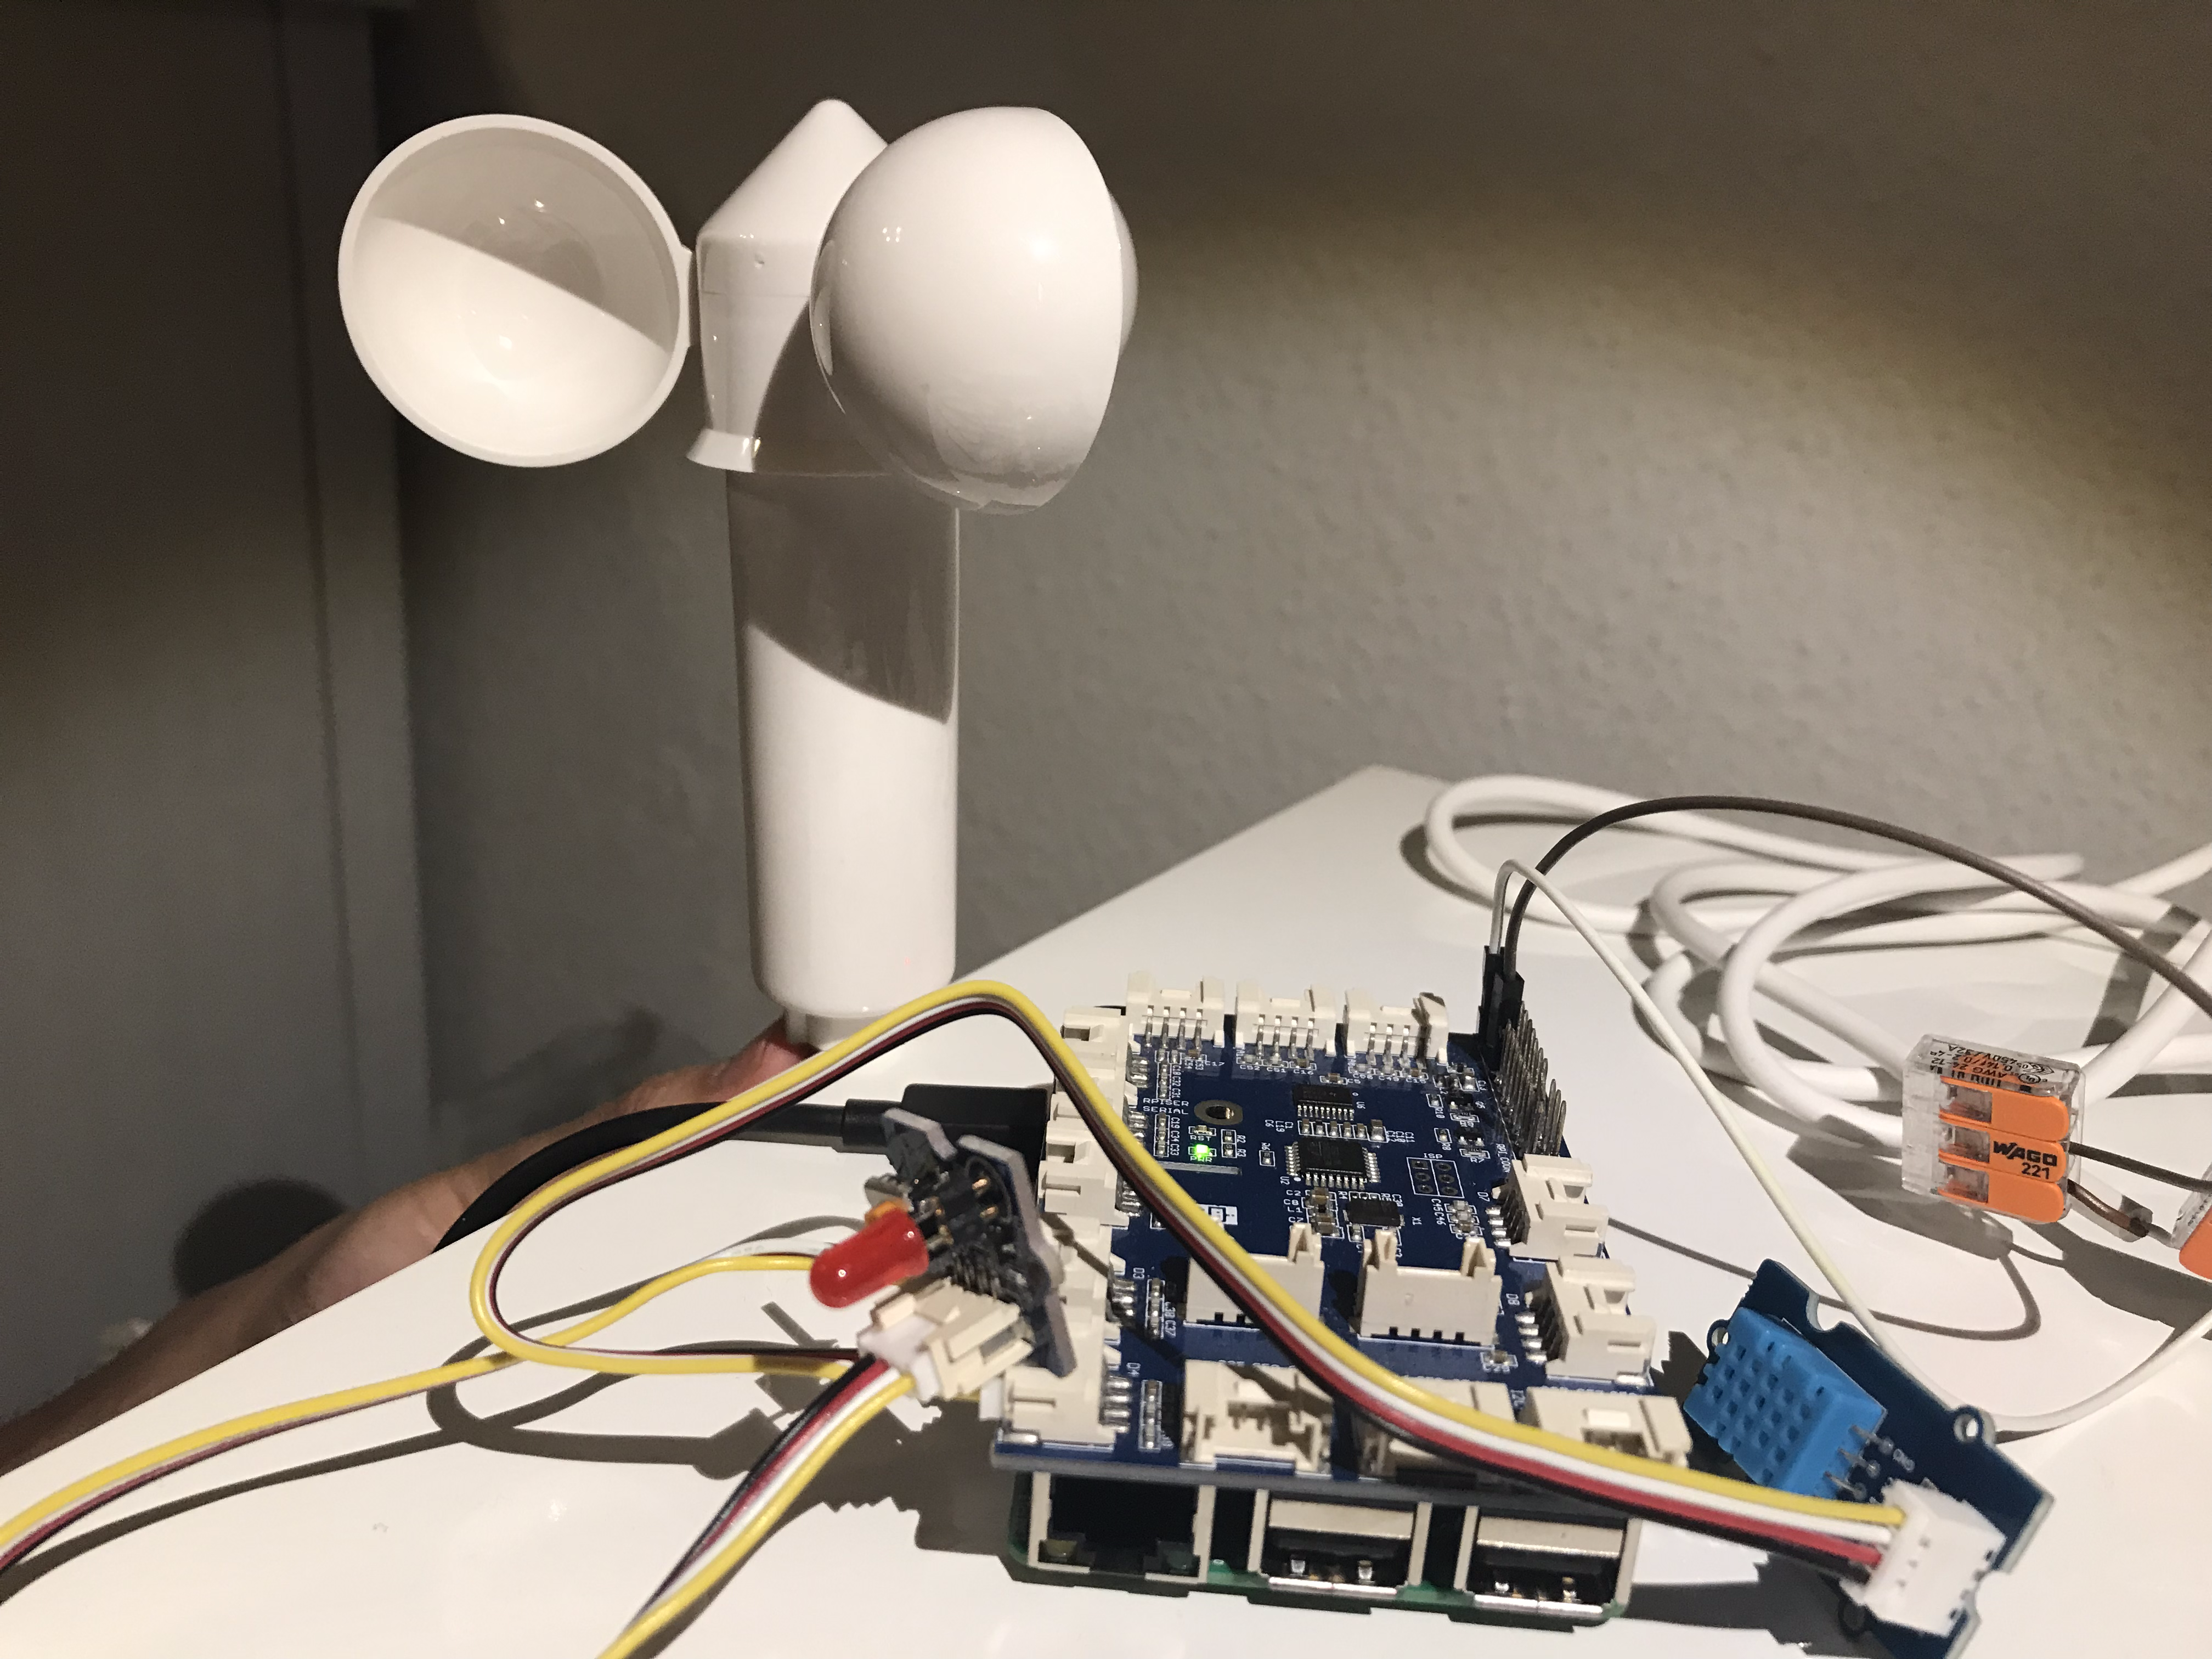
\includegraphics[width=1\linewidth]{prototype.png}
  \caption[Cyberphysisches System für die Simulation]{Cyberphysisches System für die Simulation (eigene Darstellung)}
  \label{raspi}
\end{figure}


\subsubsection{Einrichtung der Gateway Edge}

Damit die aufgenommenen Sensorwerte zur Datenhaltung an den \textit{Internet of Things Service} gesendet werden können, muss ein Gateway existieren. Doch anstatt die vordefinierten Cloud Gateways im \textit{IoT Service Cockpit} zu nutzen, wird für den Prototypen ein lokales Edge Gateway des \textit{REST}-Protokolls mit Hilfe der \textit{Internet of Things Edge Platform} konfiguriert. Zunächst wird aus dem SAP Software Center eine Konfigurationsdatei heruntergeladen, welche auf dem Raspberry Pi lokal gespeichert wird. Mit dem Befehl \textit{./build.sh REST} werden weitere Konfigurationsdateien erzeugt, um die Verbindung zu dem Host des Internet of Things Service herzustellen. In der Datei \textit{config\_gateway\_rest.xml} wird der Endpunkt für den Datentransfer in einer \textit{ConnectionAddress} definiert und eine \textit{GatewayAlternateId} definiert.

\begin{lstlisting}[caption= Gateway-Verbindung zur Cloud]
  <cnf:address>https://5075f8b9-866e-4a4b-82f8-74687b72f1ab.eu10.cp.iot.sap:443/5075f8b9-866e-4a4b-82f8-74687b72f1ab/iot/core/api/v1/tenant/988439498</cnf:address>
  <cnf:gateway gatewayAlternateId="1122334455667788">
\end{lstlisting}
Als Serveradresse des Edge Gateways wird die IP-Adresse des Raspberry Pi angegeben. Somit ist die Zieladresse für die Sensordaten zum Beispiel:

\begin{lstlisting}[caption= Zieladresse für Sensorwerte]
  https://192.168.178.52:8699/measures/<deviceAlternateId>\end{lstlisting}

\noindent Abschließend benötigt die Gateway-Registierung einen \textit{private Key im pem-Format}.

\begin{lstlisting}[caption= GET-Anfrage für einen Client-Key]
curl -X GET "https://5075f8b9-866e-4a4b-82f8-74687b72f1ab.eu10.cp.iot.sap/5075f8b9-866e-4a4b-82f8-74687b72f1ab/iot/core/api/v1/tenants/988439498/gatewayRegistrations/clientCertificate/pem\end{lstlisting}

\noindent Nach dem Starten des Gateways auf dem Raspberry Pi mit dem Befehl \textit{./gateway.sh} wird folgendes Gateway initialisiert:

\begin{lstlisting}[caption= Gateway-Eigenschaften]
  {
  "id": "2019161729",
  "alternateId": "1122334455667788",
  "protocolId": "rest",
  "name": "IoT Gateway REST",
  "type": "edge",
  "creationTimestamp": 1571741372988,
  "status": "online",
  "version": "4.42.0",
  "operatingSystem": "Linux;4.19.75-v7+;arm"
}\end{lstlisting}

\subsubsection{Registrierung der Geräte}

Bevor die Daten von der SAP Cloud Platform aufgenommen werden können, muss eine Instanz eines Gerätetypen erstellt werden. Die Registrierung folgt dem vordefinierten Datenmodell aus Abbildung \ref{fig:devicemodel} und wird mit POST-Anfragen an die \textit{Device Management API} durchgeführt. Zunächst wird mit die \textit{Capability wind\_1} vom Typ \textit{measure} erstellt. Der Capability werden die \textit{Properties wind\_speed, temperature, humidity, pressure und airtight} zugeordnet. Damit das Gerät Befehle empfangen kann, wird außerdem die Capability \textit{commands\_test} vom Typ \textit{command} erstellt. Anschließend werden beide Capabilities einem Sensortypen zugeordnet. Um jedoch eine Geräteinstant erzeugen zu können, muss eine
mit SAP Cloud Platform Internet of Things und Device Model hier erstellen und als Bild einfügen und außerdem zunächst auf Tenants und User eingehen und Einrichtungs des Services generell erklären mit eventuell den Message Processings
und Gateways etc



\subsubsection{Senden der Daten an die Cloud}

\begin{lstlisting}
============================================
Reading sensor data ...
{'capabilityAlternateId': '1234', 'measures': [{'temperature': '19.0'}, {'wind_speed': '1.12102078977'}, {'pressure': '1010'}, {'humidity': '70.0'}, {'airtight': '1.2'}], 'sensorAlternateId': '1234'}
==> HTTP Response: 202
\end{lstlisting}

\subsubsection{Erstellen des digitalen Zwillings}

\paragraph{Regeln, Ereignisse, Aktionen}

AWS, Events, LED Commands und Destinations
\subsubsection{Visualisierung mit einer UI5-Applikation}


\subsubsection{Zusammenfassung Implementierung}

\newpage




